%--------%
%->> Section 4.3: 任务执行与数据管理
%------------------%

\section{任务执行与数据管理}

前两节分别说明了平台的总体架构，以及第三章三类方法在系统中的实现方式。本节进一步介绍任务在平台中的组织形式，以及相关数据在执行过程中的管理方式。这里主要涉及两方面内容：其一，工作区、任务与知识库之间的数据关系；其二，离线知识构建任务与在线诊断任务的执行过程。

平台以工作区作为任务运行的基本单元。无论是在线诊断还是离线知识构建，系统都会先创建独立工作区，并在其中初始化该任务所需的故障实例信息、接口地址、当前 SOP 和任务标识等上下文。通过这种方式，一次任务执行过程中涉及的数据、状态与结果都被统一组织在同一工作区之下，从而便于后续管理、复现与结果回流更新。

图\ref{fig:system_data_model}给出了工作区、任务与 SOP 之间的数据关系。

\begin{figure}[htbp]
    \centering
    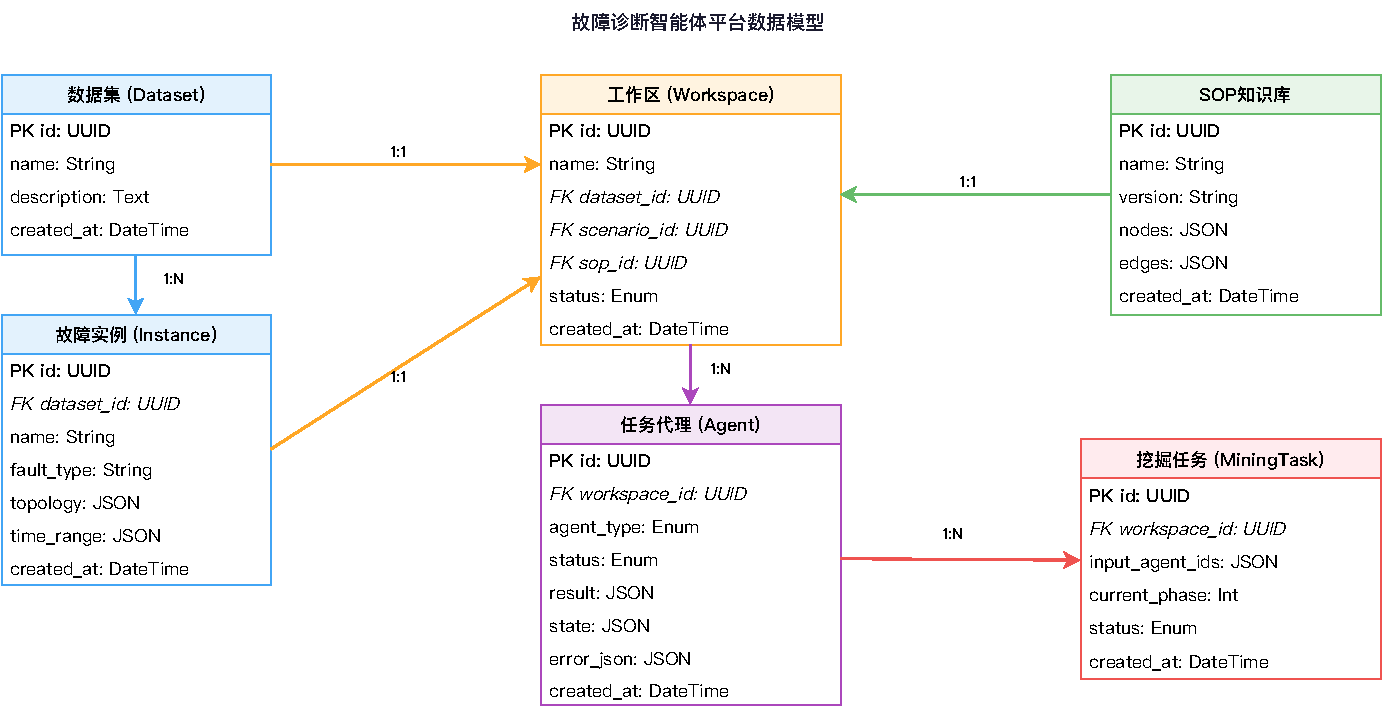
\includegraphics[width=0.92\textwidth]{Figures-Src/Chap4-System/data-model/chart.pdf}
    \bicaption{\enspace 工作区、任务与SOP的数据关系}{\enspace Data Relationships Among Workspaces, Tasks, and SOPs}
    \label{fig:system_data_model}
\end{figure}

如图\ref{fig:system_data_model}所示，系统中的数据模型包含六个核心实体。Dataset（数据集）保存原始数据的基础信息；Instance（故障实例）记录数据集下单次故障的可观测数据及其故障信息，同一数据集可以对应多个故障实例；Workspace（工作区）将数据、故障实例和 SOP 组织到一次任务执行中，并通过外键唯一关联一个数据集、一个故障实例和一个 SOP 知识库；SOP Knowledge Base（SOP 知识库）以有向图形式保存 SOP；Agent（任务代理）记录一次具体任务的执行状态与任务类型；MiningTask（挖掘任务）记录离线规则整理相关任务。通过这一数据结构，同一故障实例可以在在线诊断和离线知识构建两个阶段挂接到统一的工作区上下文下，从而便于共享故障实例信息与历史结果。

从任务组织方式看，平台中的 Agent 可分为两类。第一类是主任务代理，分别加载 \texttt{Diagnosis-Skill}、\texttt{Exploration-Skill} 和 \texttt{Rule-Skill}，负责在线诊断、离线探索和规则整理三类主任务；第二类是观察 subagent，其不承担完整任务流程，仅在主任务需要补充观测数据时被临时创建，用于调用 \texttt{Observe MCP} 执行专项查询。这种划分方式使流程控制与数据采集相互分离，也避免主任务会话长期携带大量观测工具上下文。

离线知识构建任务的执行过程可以概括为以下三个环节：

\begin{enumerate}[label=（\arabic*）]
    \item \textbf{探索轨迹生成。}
    用户在前端发起 SOP 构建任务后，后端首先创建工作区，并启动 \texttt{Exploration-Skill}。在执行过程中，\texttt{Exploration-Skill} 围绕当前 SOP 进行多轮探索，决定每一步应检查的节点以及需要补充的证据；若需要访问指标、日志或链路数据，则创建观察 subagent，由其通过 \texttt{Observe MCP} 完成相应查询。探索过程中形成的判断路径和观测结果会持续保存至轨迹存储。

    \item \textbf{规则整理与决策单元提取。}
    在轨迹生成完成后，后端读取轨迹存储中的探索轨迹，并启动 \texttt{Rule-Skill}。该阶段主要对轨迹中的关键判断、节点跳转和结论形成过程进行拆解，完成语义归一化、决策单元提取与权重计算。第 3 章定义的四项指标 MI、DF、TD 和 EV 也在这一阶段完成计算与聚合。

    \item \textbf{SOP 增量更新。}
    \texttt{Rule-Skill} 根据高权重决策单元对原有 SOP 执行节点增删改操作，并将更新后的有向图同步至 SOP 知识库。任务完成后，系统将构建结果返回前端，从而形成一次完整的离线知识构建流程。
\end{enumerate}

在线故障诊断阶段的执行时序如图\ref{fig:online_sequence}所示，在线诊断过程可以进一步概括为以下五个步骤：


\begin{figure}[htbp]
    \centering
    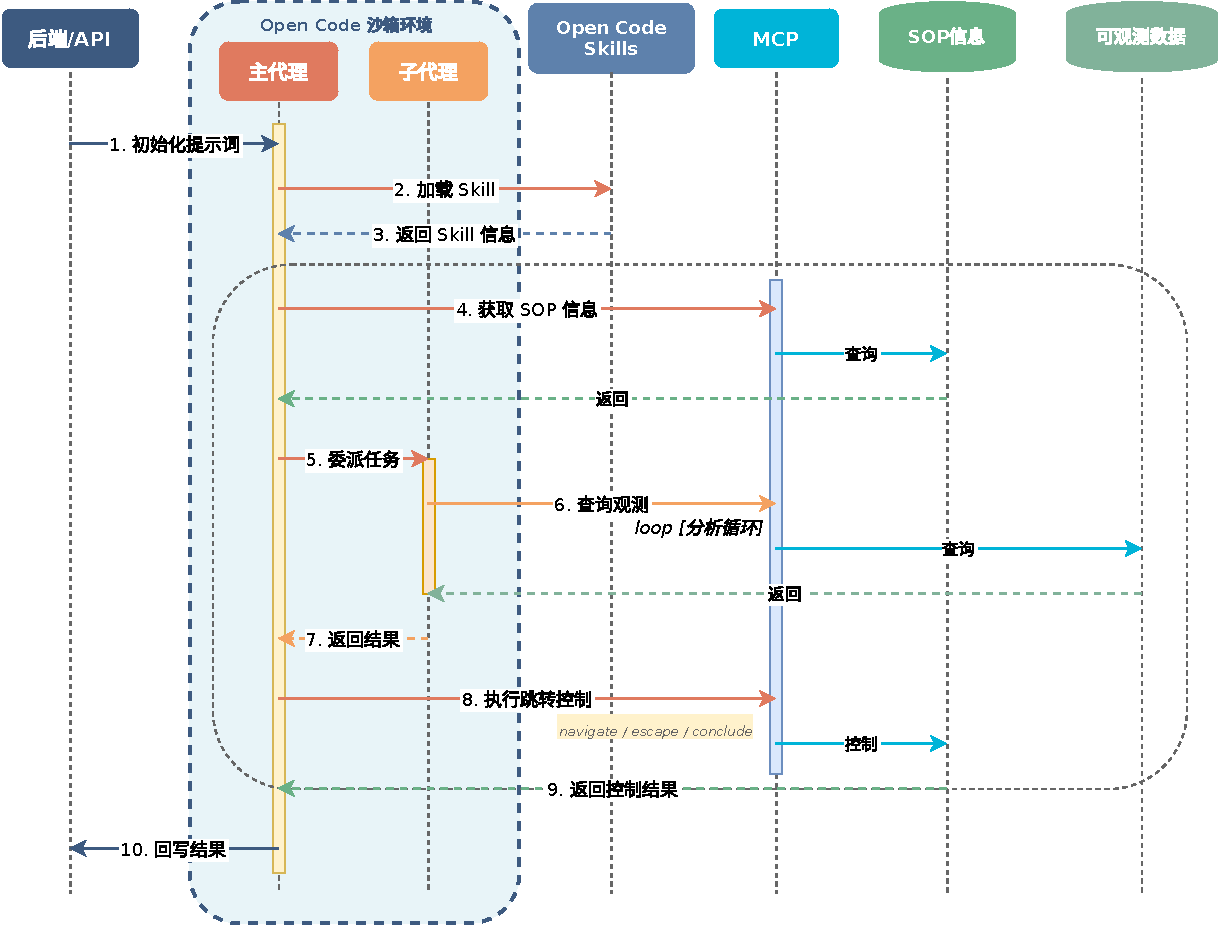
\includegraphics[width=0.98\textwidth]{Figures-Src/Chap4-System/online-diagnosis-timeline/chart.pdf}
    \bicaption{\enspace 在线诊断任务执行时序}{\enspace Execution Sequence of an Online Diagnosis Task}
    \label{fig:online_sequence}
\end{figure}


\begin{enumerate}[label=（\arabic*）]
    \item \textbf{任务初始化。}
    后端接收到告警后，首先完成故障指纹检索，获得最近邻故障簇及其候选 SOP；随后创建工作区，并在其中初始化告警信息、检索结果和候选 SOP。

    \item \textbf{诊断会话启动。}
    OpenCode 启动诊断会话并加载 \texttt{Diagnosis-Skill}，读取当前工作区中的任务上下文，并据此初始化焦点与感知域，为后续在线诊断提供起始状态。

    \item \textbf{观测证据收集。}
    当主流程需要补充观测数据时，\texttt{Diagnosis-Skill} 创建观察 subagent，由其通过 \texttt{Observe MCP} 查询所需的指标、日志和链路数据，并将结果返回主流程。

    \item \textbf{诊断路径推进。}
    \texttt{Diagnosis-Skill} 根据返回结果执行 \texttt{navigate}、\texttt{escape} 或 \texttt{conclude}，并在此过程中持续更新当前焦点、感知域和后续动作，从而推动诊断过程逐步收敛。

    \item \textbf{结果保存与回流更新。}
    诊断结论、关键证据和完整执行过程被保存至后端与数据存储层，并同步反馈到前端界面。经过后续人工审核后，相关结果还将进一步进入故障指纹更新流程和 SOP 增量更新流程。
\end{enumerate}

在上述执行机制下，工作区负责统一承载任务上下文，主 Skill 负责推进任务流程，观察 subagent 负责查询可观测数据，后端与数据存储层负责保存执行过程与任务结果。由此，离线探索、在线诊断以及后续知识更新能够在同一套任务管理与数据管理机制下协同运行。